\documentclass[10pt]{article}
\usepackage{typoday18}

\title{Spiral splines in typeface design - A case study of Manjari Malayalam typeface}

\author{ 
 Santhosh Thottingal
 \and
 Kavya Manohar
}
 

\begin{document}

\maketitle

\begin{abstract}

Manjari typeface was an experiment to use spiral splines to define the curves of Malayalam glyphs. It was a milestone in the progression of script towards maximally rounded glyphs. The script has been evolving from its rectangular characteristics in the early days of metallic types to the circular characteristics of popular digital fonts. 

The design of curves in Manjari are theoretically based on the PhD thesis by Raph Levien - ``From Spiral to Spline: Optimal Techniques in Interactive Curve Design” \cite{levien}. The design process relied almost entirely on the spiro toolbox developed by Levien himself, available as free software library in Inkscape vector graphics editor.

The use of spiral spline curves resulted in shapes that are extra smooth. The spiral smoothness of curves are complemented by rounded terminals which gives very soft feeling for the eyes. The rigidness of geometric fonts is completely avoided giving a good humanist identity. The curve perfection resulted in negative spaces that aquired beautiful leaf and drop shapes between the bowls and loops of the script. 

In this paper we present the design principles and aesthetic concepts behind this font along with a perspective on the evolution of script aesthetics from the ancient writing systems, through early and contemporary printing to digital fonts. We will also discuss the popularity and adoption of Manjari in the digital as well as print media.
\end{abstract}

\textbf{Keywords:} Malayalam, Script, Spirals, Opentype, Typeface, Digital Typography

\section{Introduction}

Malayalam script, since its evolution from Brahmi\footnote{\url{https://www.britannica.com/topic/Brahmi}} writing style through Vattezhuthu and Grantha\footnote{\url{https://www.britannica.com/topic/Grantha-alphabet}} writing systems to the digital typefaces of modern era, has undergone a lot of changes. The noticeable aesthetic feature of contemporary script is its loops and curly strokes. Horizontal symmetry for many letters like {\rachana {ക, ത, ന}} became an identity for the script. Manjari Malayalam typeface utilises spiral shapes to accentuate these features that resulted in its aesthetic acceptance. A sample of text rendered in Manjari typeface is shown in Figure \ref{wordcloud}.


\begin{figure}[h!]
	\centering
	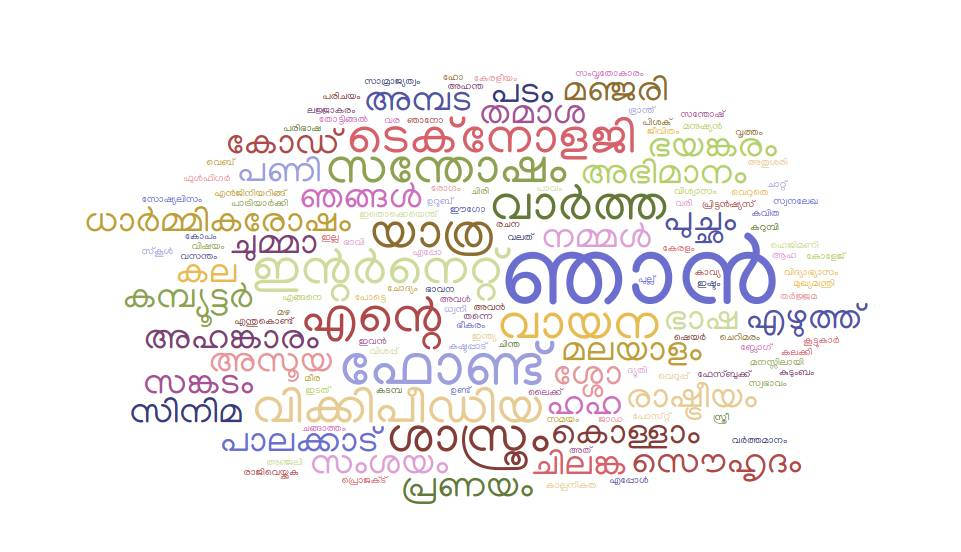
\includegraphics[width=\textwidth]{images/wordcloud.jpg}
	\caption{Text rendered in Manjari typeface}
	\label{wordcloud}
\end{figure} 

\section{Evolutionary Path of the script}

Samples of copper plate inscriptions and palm leaf manuscripts show that the letters were never perfect rounds, but rather rectangular or elongated curves. The sample shown in Figure \ref{vattezhuthu} is inscription from Tharisappalli copper plates dating back to 849 AD.


\begin{figure}[h!]
	\centering
	\includegraphics[width=0.6\textwidth]{images/Tharisappalli_copper_plates.jpg}
	\caption{Copper plate inscription in Vattezhuthu.}
	\label{vattezhuthu}
\end{figure} 


The rectangular nature of the script was its characteristic during the early days of printing. The first ever printed Malayalam book was Samkshepavedartham, printed in Rome using movable types in 1772. Sample pages of the book is shown in Figure \ref{Samkshepam}. 


\begin{figure}[h!]
	\centering
	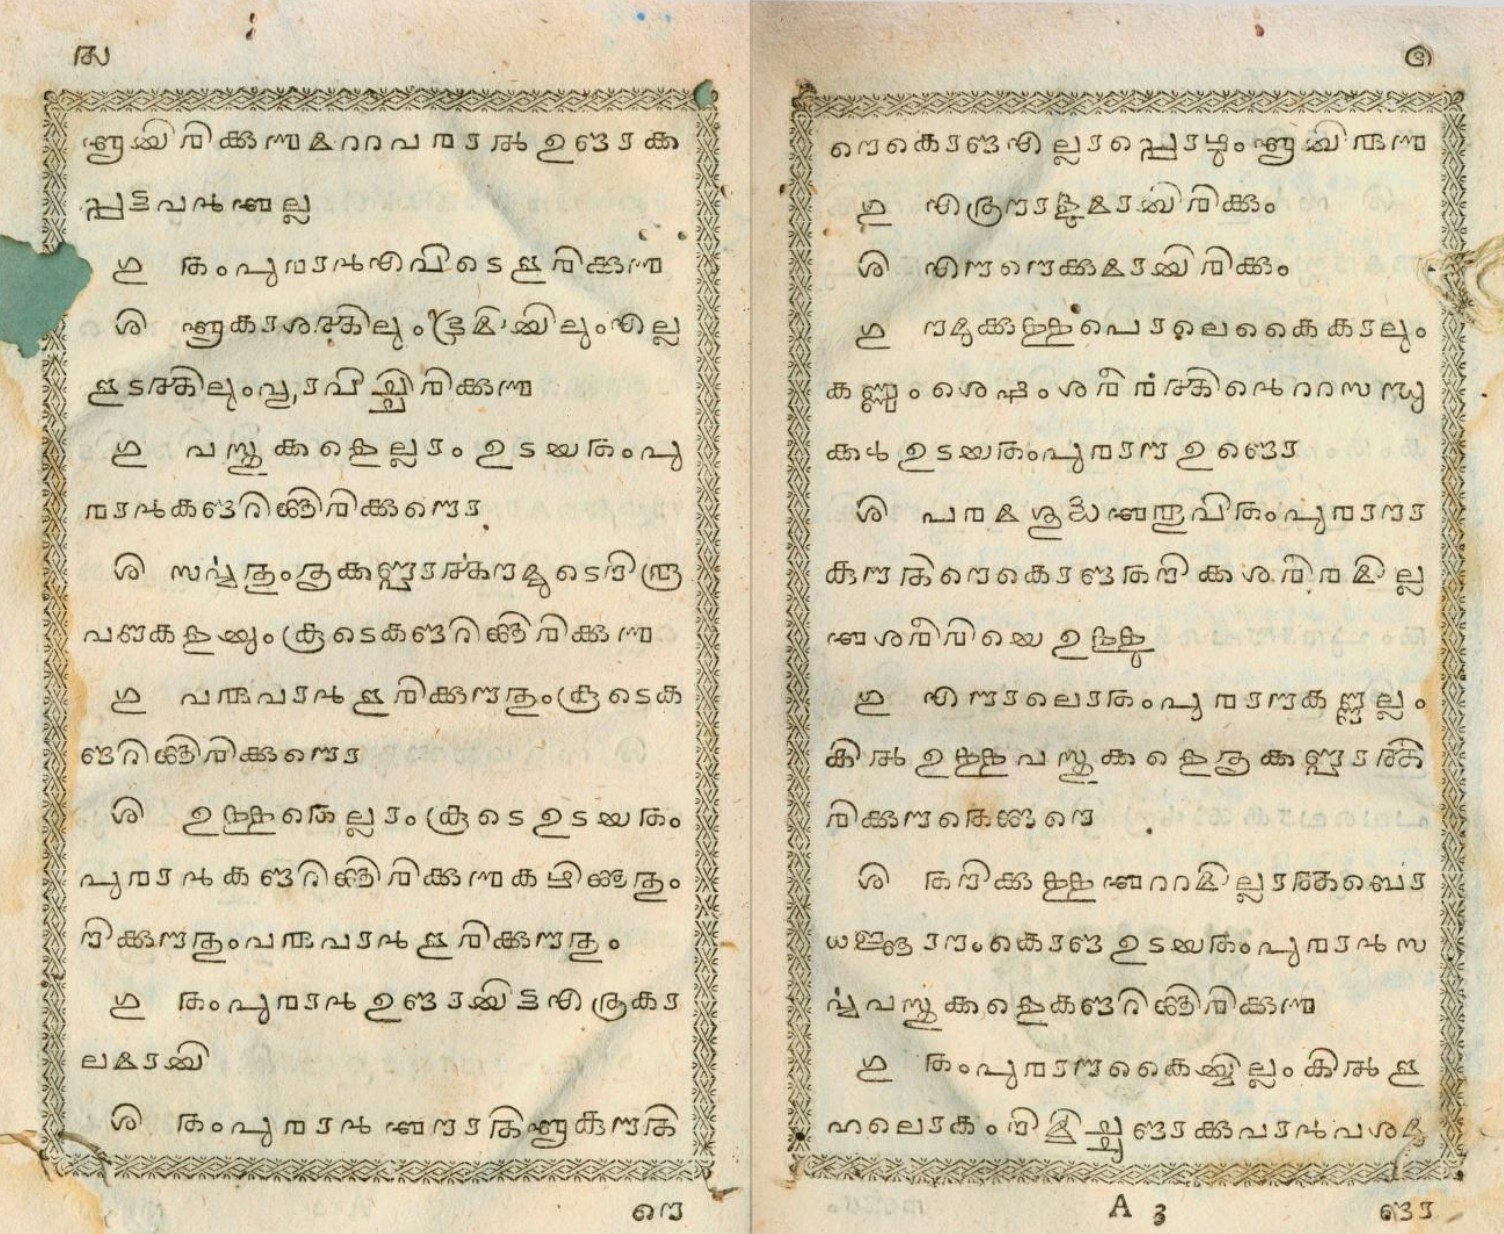
\includegraphics[width=0.8\textwidth]{images/samkshepavedartham1772.png}
	\caption{Samkshepavedartham-1772 shows rectangular nature of glyphs in early print}
	\label{Samkshepam}
\end{figure} 

Next remarkable event in history of Malayalam typefaces occurred when movable types were casted natively in Kerala, India during 1829 by an Anglican Missionary Benjamin Bailey\cite{babucherian} for CMS Press, Kottayam, Kerala. These metal types were close to perfect round and the popularity of books from this press started to give uniform height proportions to the script. According to Gupthan Nair, Bailey's contributions as a typographer made the curvy style of the Malayalam script popular\cite{gupthannair}. See the most impactful output from the CMS Press Kottayam in Figure.\ref{newtestament}, a translation of the Bible.


\begin{figure}
	\centering
	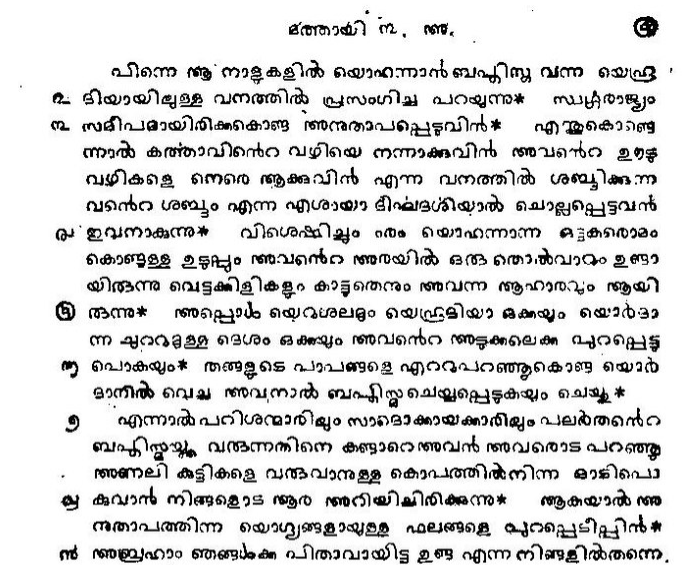
\includegraphics[width=0.8\textwidth]{images/newtestament1829.png}
	\caption{New Testament - 1829}
	\label{newtestament}
\end{figure}

The acceptance of this style of roundness can be easily understood when a fine handwriting is often referred as `{\manjari {അവൾക്കു നല്ല ഉരുണ്ട കയ്യക്ഷരമുണ്ട്} }' (She has a fine round shaped handwriting).


\subsection{Digital typefaces}

Digital typefaces of Malayalam script introduced during after 1990 were non-standard ones. These fonts were based on ASCII encoding, with script mapped to Malayalam glyph set. Malayalam was not encoded in Unicode until 2001. This non-standard work around became popular in the publishing industry, and a huge variety of typefaces were designed for this technology. The fonts that got popular in regular printing were mostly rounded. See Figure.\ref{maltextbook}

\begin{figure}
	\centering
	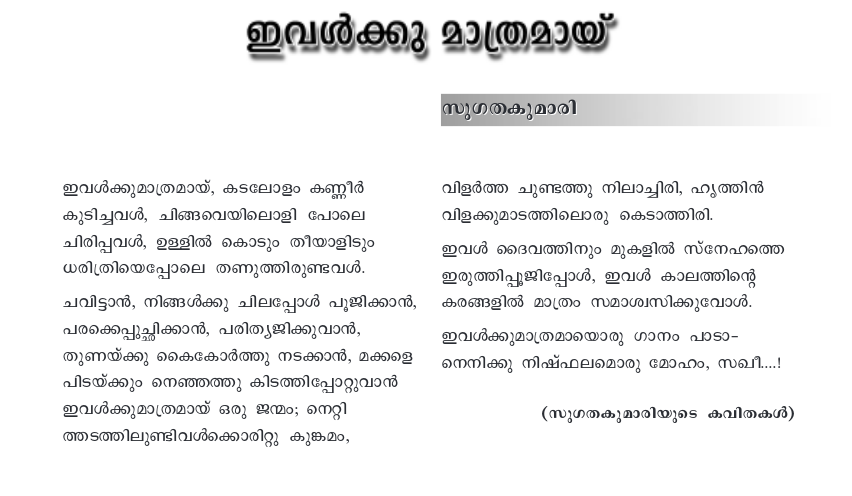
\includegraphics[width=0.8\textwidth]{images/2011-Malayalam-Textbook.png}
	\caption{Malayalam Text book in 2011. ASCII based font.}
	\label{maltextbook}
\end{figure}

 
 The most popular unicode fonts since their release in the late 2000s: Rachana, Meera and Anjali continued to follow roundness as their glyph characteristic. 

Manjari\footnote{Available at \url{https://smc.org.in/fonts/\#manjari}. The source code is published under open font license at \url{https://gitlab.com/smc/manjari}} is a typeface designed by Santhosh Thottingal. This font was released in July 2016 and immediately gained wide popularity among Malayalam speakers. The curves in Manjari are designed to follow a spiral shaped path between its control points and the terminals are rounded. %See Figure.\ref{manjari-ka}.

%\begin{figure}
%	\centering
%	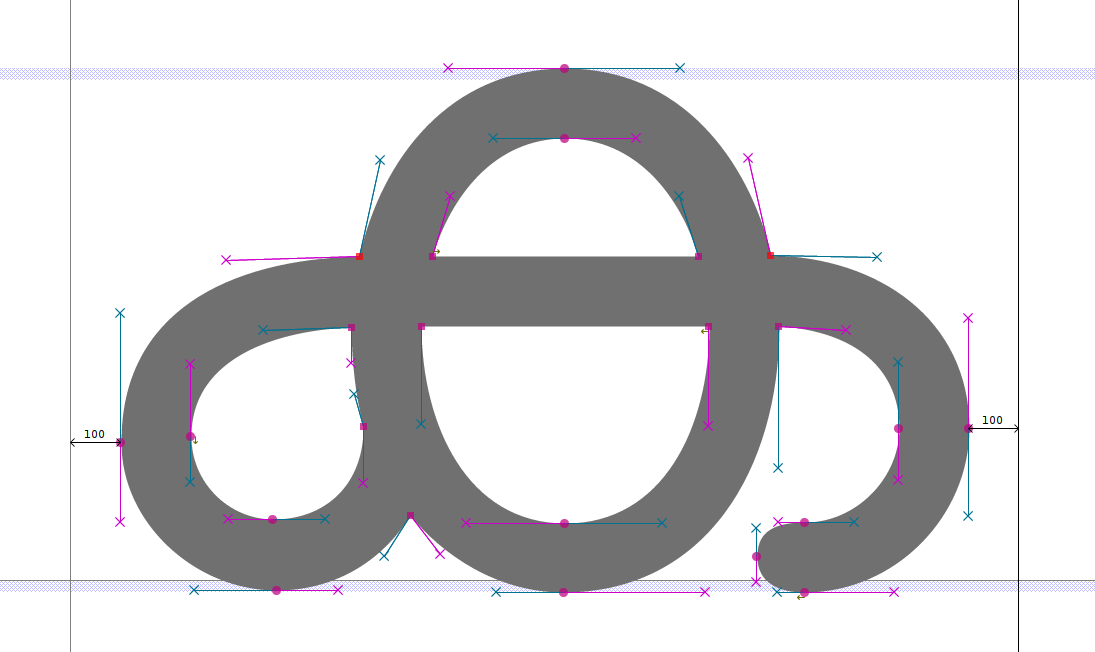
\includegraphics[width=0.8\textwidth]{images/Manjari-Ka.png}
%	\caption{Drawing of letter {\manjari ക} in Manjari font}
%	\label{manjari-ka}
%\end{figure} 
 
 The following section describes mathematics of the curves that define Manjari. 
 


\section{Curve Interpolation by Spiral splines}

Curves that passes through control points in a sequence can be termed interpolating splines. A good interpolating spline is a smooth curve that results from sparse control points. There are a huge variety of interpolating curves that include spiral splines, minimum energy curves, log aesthetic curves etc. As mentioned earlier, the nature of smooth interpolating splines have been studied by Ralph levien in his thesis, ``From Spiral to Spline: Optimal Techniques in Interactive Curve Design”\cite{levien}.

According to Levien, spiral spline interpolating curves have certain characteristics which make them particularly suitable for two dimensional curve fitting.
\begin{itemize}
	
	\item Roundness Property: When spiral spline curves are used for interpolation, three data points on a circular path would yield that exact circle after interpolation.
	\item Extensionality Property: When a new control point is introduced on the interpolated spline between two points, the curve shape would be preserved.
\end{itemize}

The continuity in variation of the curvature of a curve is an indicator of its fairness. Parameterized polygons are continuous only in $G^0$, their curvature has a first derivative everywhere, the basic property of connected curves. Spline curves with $G^1$ continuity have a second derivative everywhere. Spiral splines can be defined with $G^2$ continuity has a third derivative everywhere indicating very smooth variation in curvature. 
 
Levien proposes that \textbf{every curve segment in a second order continuous interpolating spiral spline between adjacent control points can be cut from an Euler spiral subjecting to rotation, scaling, translation and mirror image transformations}. He calls Euler spiral as the generating curve for spiral splines. Euler spiral has a curvature that changes linearly with its curve length. See Figure.\ref{eulerspiral} for a Euler spiral.


\begin{figure}
	\centering
	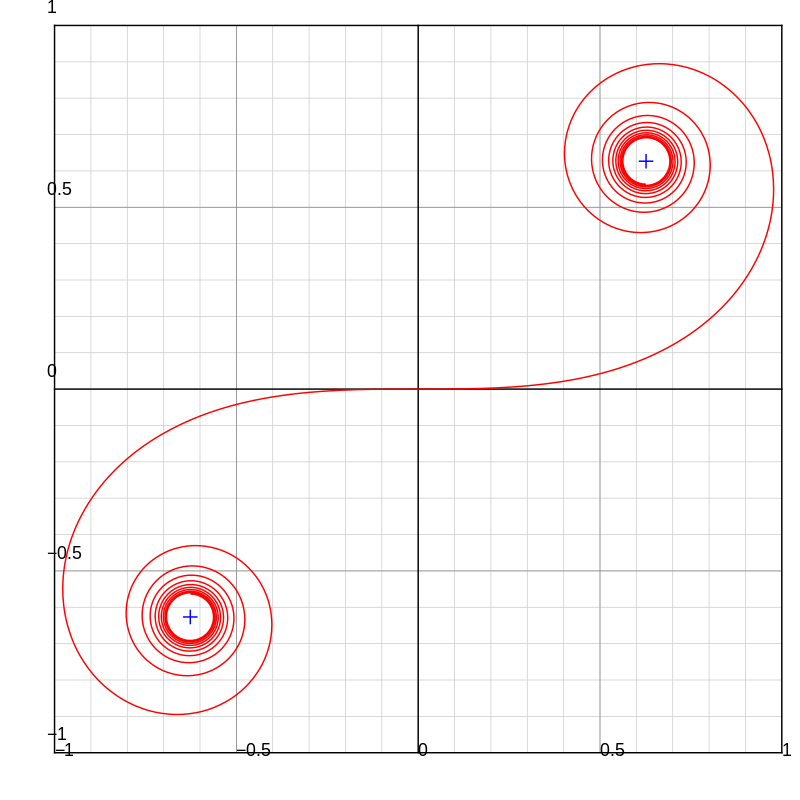
\includegraphics[width=0.8\textwidth]{images/Euler_spiral.png}
	\caption{Euler Spiral}
	\label{eulerspiral}
\end{figure}


The Inconsolata monospace humanist latin font known for its clean lines and elegant design by Levien himself is based on this theory.

\paragraph{Fonts variants by interpolation}
Many interpolating splines in the literature are used for generating variations in fonts, rather
than a single static shape. Since fonts are desired in a wide range of weights, one of the more
common applications is to generate these continuously. One of the most straightforward techniques,
pioneered by Ikarus [42], is to start with two masters with similar structure, representing thin
and thick extremes, and linearly interpolate the positions of the control points between the two.
Then, an interpolating spline is fit through these control points. Note that there are two senses of
interpolation here – one for the control points, another for the spline." \cite{lamport94}

\section{Design process}

The design of Manjari font was done using free software tools in GNU/Linux operating system. The drawing was done in Inkscape using the Spiro tool\footnote{Spiro library. Spiro is a toolkit for curve design, especially font design, created by Raph Levien. It is integrated with Inkscape and Fontforge. \url{http://www.levien.com/spiro/}}, which implements the optimal curve generation technique outlined by Raph Levien. figure \ref{design-1}, \ref{design-2}, \ref{design-3} and \ref{design-4} illustrates the process.

\begin{figure}[h!]
	\centering
	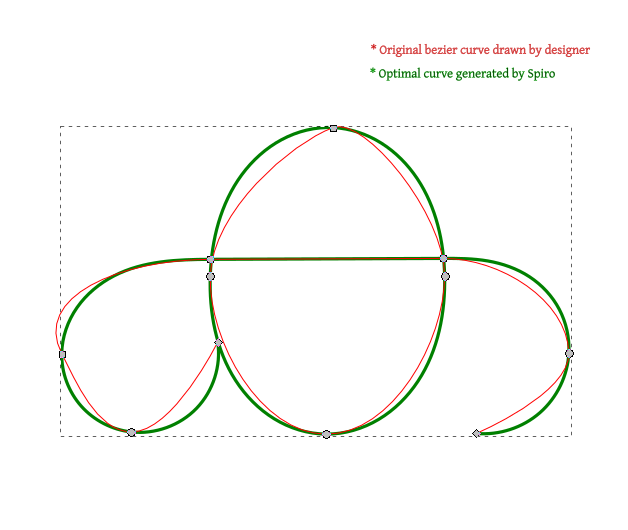
\includegraphics[width=0.8\textwidth]{images/design-1-spiral.png}
	\caption{Designer draws the bezier path. Spiro tool calculates the optimal curve. Designer adjusts the nodes till the glyph shape is achieved.}
	\label{design-1}
\end{figure}

\begin{figure}[h!]
	\centering
	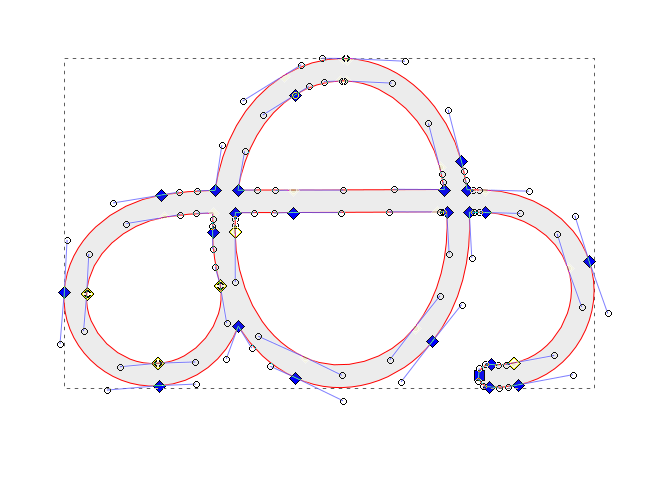
\includegraphics[width=0.8\textwidth]{images/design-2-stroke-to-path.png}
	\caption{The stroke converted to path with desired stroke width. Now this is draft of cubic bezier outline of glyph}
	\label{design-2}
\end{figure}

\begin{figure}[h!]
	\centering
	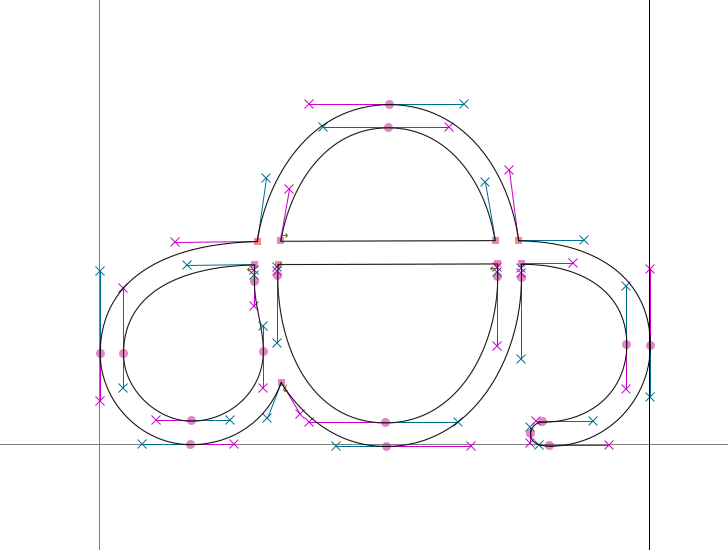
\includegraphics[width=0.8\textwidth]{images/design-3-cubic-bezier-in-font-editor.png}
	\caption{A font editor simplifies and clean up the nodes, defines glyph name, bearings.}
	\label{design-3}
\end{figure}

\begin{figure}[h!]
	\centering
	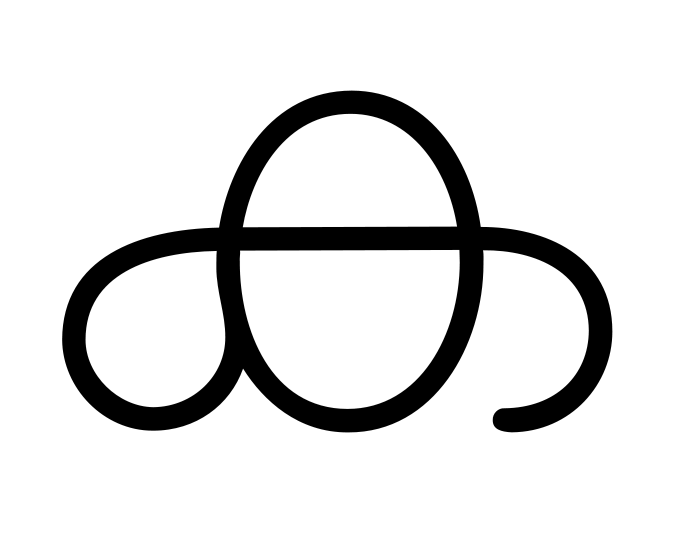
\includegraphics[width=0.8\textwidth]{images/design-4-final.png}
	\caption{Final glyph}
	\label{design-4}
\end{figure}

Manjari is equal thickness typeface. So bold, thin variants prepared by just varying the stroke with in Inkscape, while stroke is controlled by the curves from Spiro. The outline terminals were set to use round shapes, that complements the smoothness in outlines.

\section{Manjari and its Spiral features - 35 \% of content}

Curves Defined by spiral interpolation

Round edges: Smooth feeling

Equal widtn stroke

\newpage

\section{Specimen}

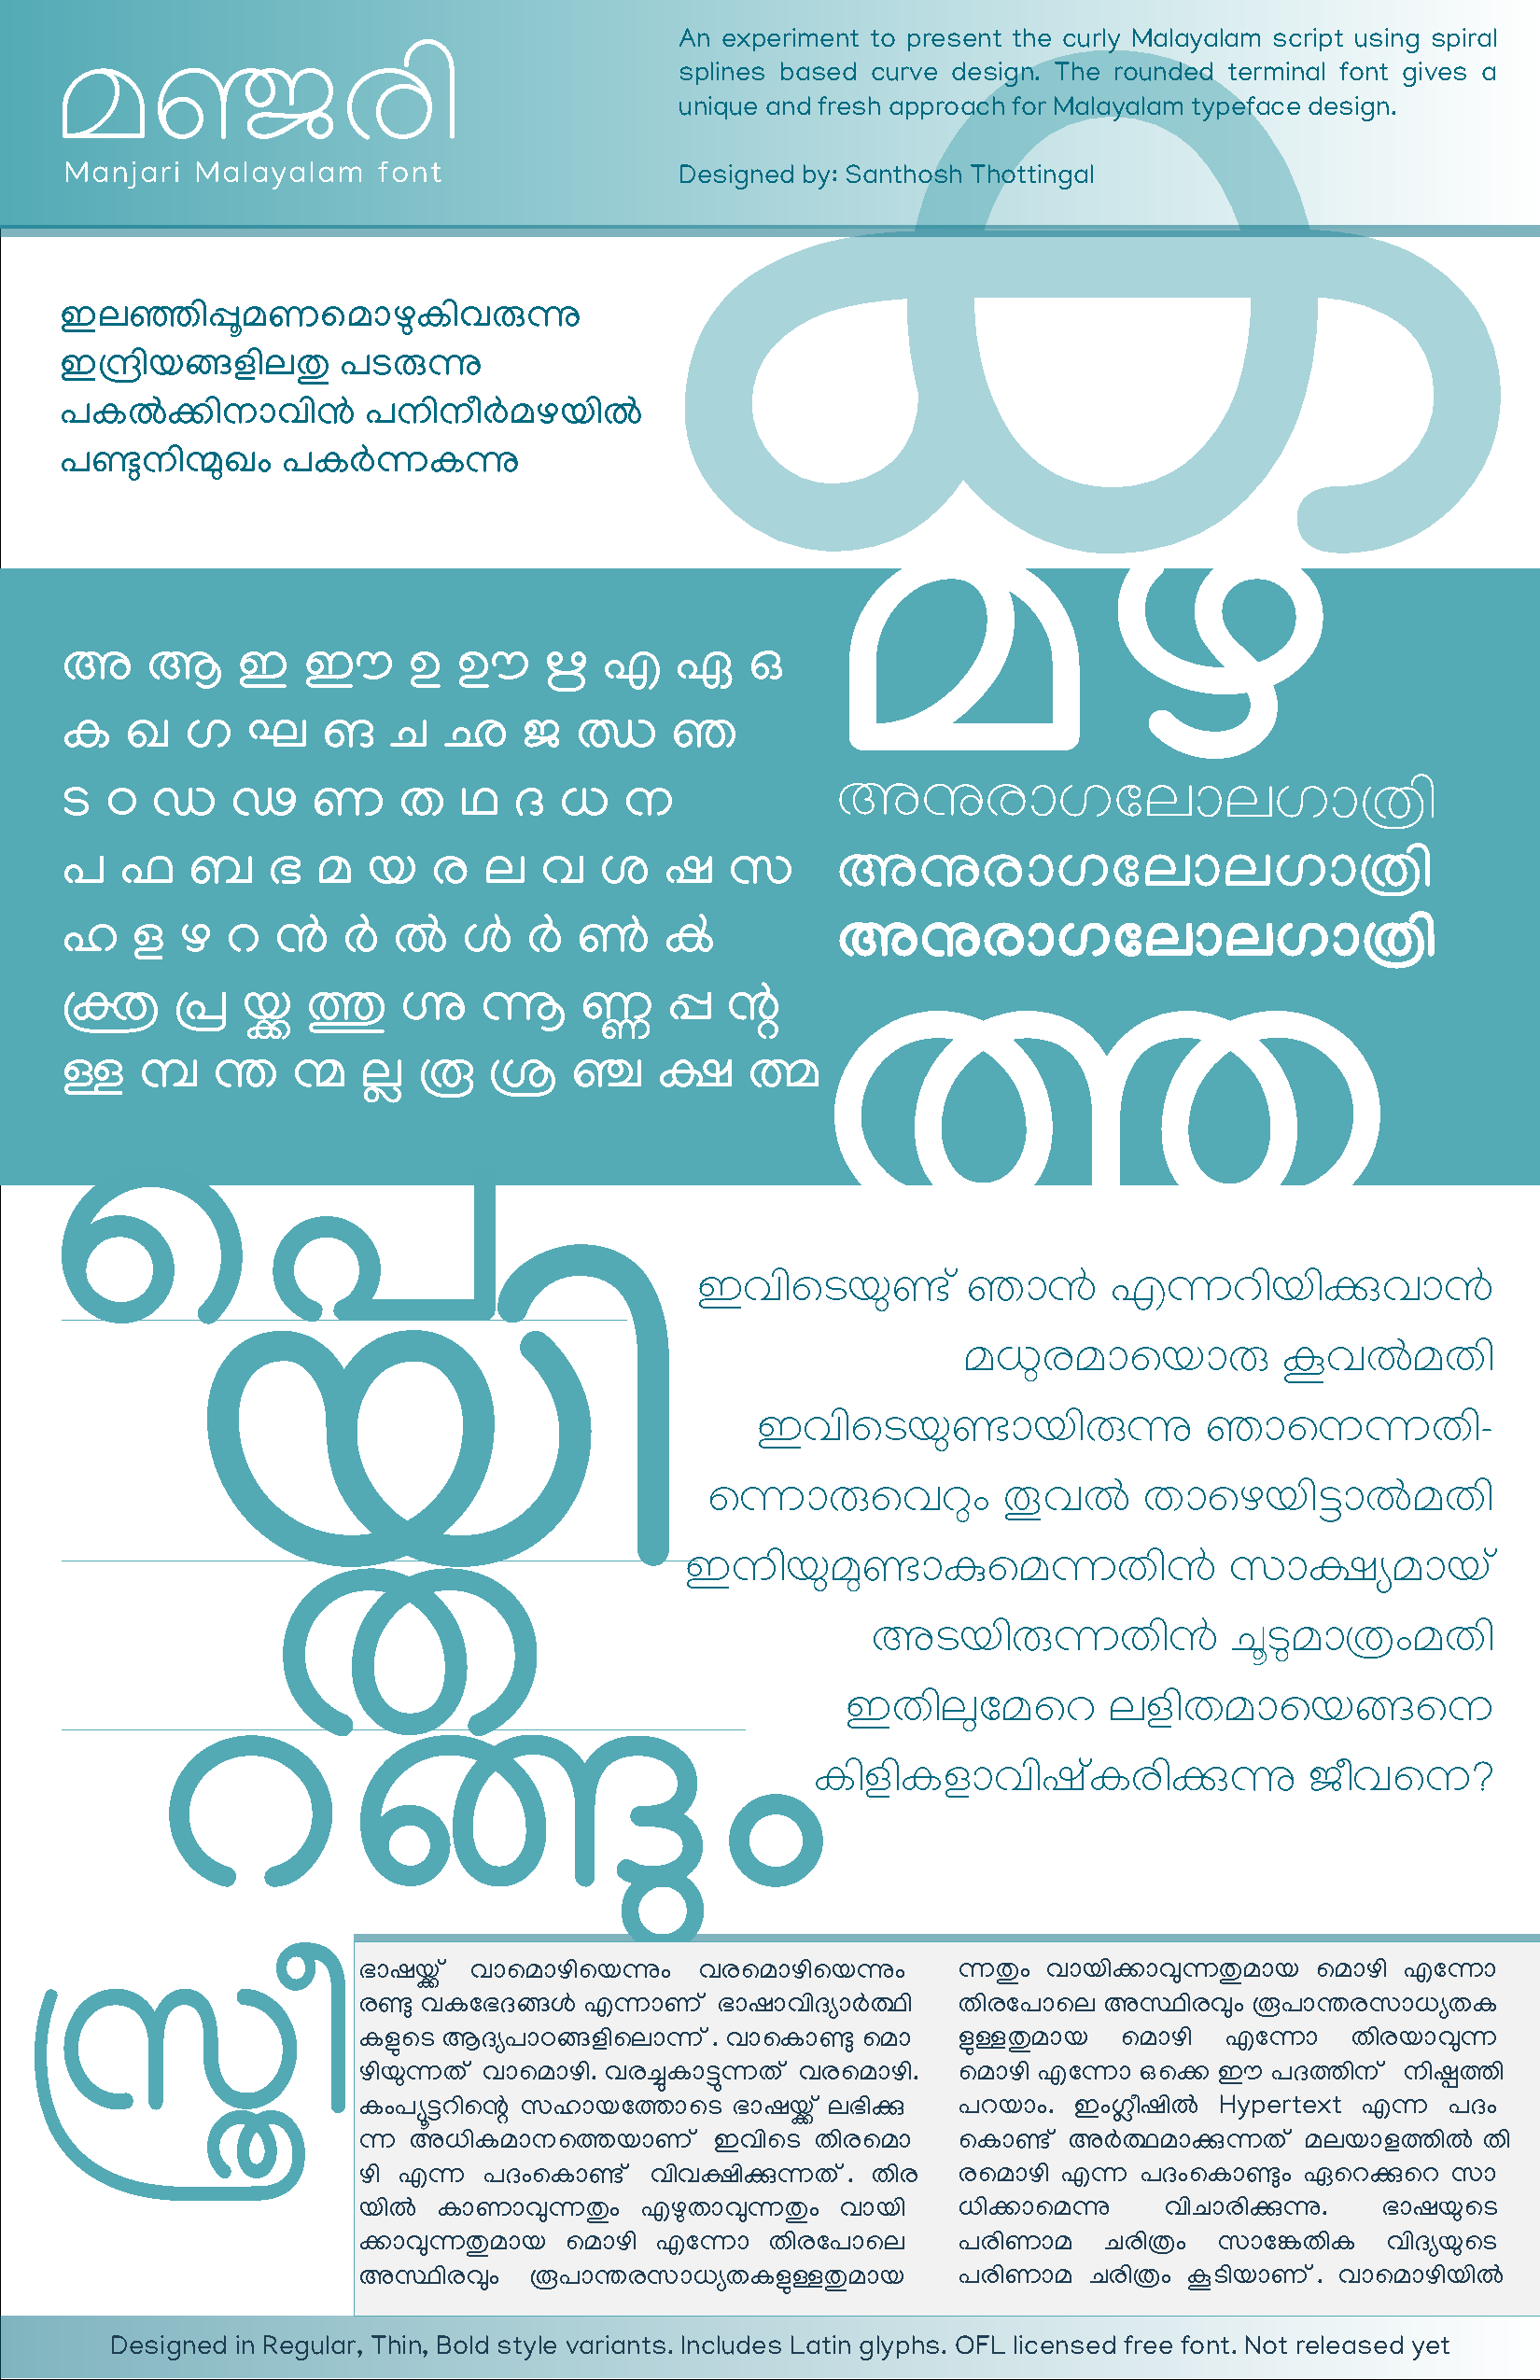
\includegraphics[width=\textwidth]{images/Manjari-Specimen.pdf}

\section{Conclusion}
sds

\begin{thebibliography}{11}
	\bibitem{levien} Raphael Linus Levien, \textit{From Spiral to Spline: Optimal Techniques in Interactive Curve Design}, EECS Department, University of California, Berkeley, 2009
	\bibitem{babucherian} Babu Cheriyan, \textit{Benjamin Bailiyum Malayala Sahithyavum} {\manjari{(ബെഞ്ചമിൻ ബെയിലിയും മലയാള സാഹിത്യവും}) }, Mahatma Gandhi University, Kottayam, 2008
	\bibitem{gupthannair} S. Gupthan Nair, \textit{Gadyam Pinnitta Vazhikal}{\manjari{ (ഗദ്യം പിന്നിട്ട വഴികൾ)} }, DC Books, Kottayam 

	
\end{thebibliography}


\end{document}
